\chapter{Related works}

\section{ROS2}

ROS2\cite{ROS2} (Robot Operating System 2) is not an operating system (despite its name), it is a framework which helps us to create robotic systems.

Nodes can be created to solve basic tasks (for example handling the differential drive), they can communicate with each other via topics (it is a publish-subscribe communication). If we desire to execute time consuming commands it is advised to use actions instead of simple nodes. Actions contain a client node, a server node, a goal and result service, and a feedback topic. Services are different than topics because they implement a client-server communication with request and result topics embedded in them. The client can specify a goal to the server which sends feedback periodically when executing the request. At the end the client can get the result on the result service. An action can be used for navigation because it could take a long time and we want to be informed about the progress of the navigation or the status of the robot (e.g position, orientation, speed). 

One of the most exciting advantage of using this framework is that we can create nodes in C++ and Python in the same system, they will be able to work with each other with the help of topics. The reason this works is that a topic can only contain one of the several strict message types and these are exactly the same in both programming languages.

\section{Turtlebot4}

At Nokia we worked on a Turtlebot4\footnote{\url{https://clearpathrobotics.com/turtlebot-4/}} to achieve our goals. It is based on an iRobot® Create3\footnote{\url{https://edu.irobot.com/what-we-offer/create3}} mobile base and it is equipped with lots of tools and sensors. Create3 is a robot vacuum cleaner's base made for educational use by iRobot. It contains the differential drive, the IR proximity sensors in the front and the docking station for charging. All in all it can be used to build more complex mobile robots.

\begin{figure}[H]
    \centering
    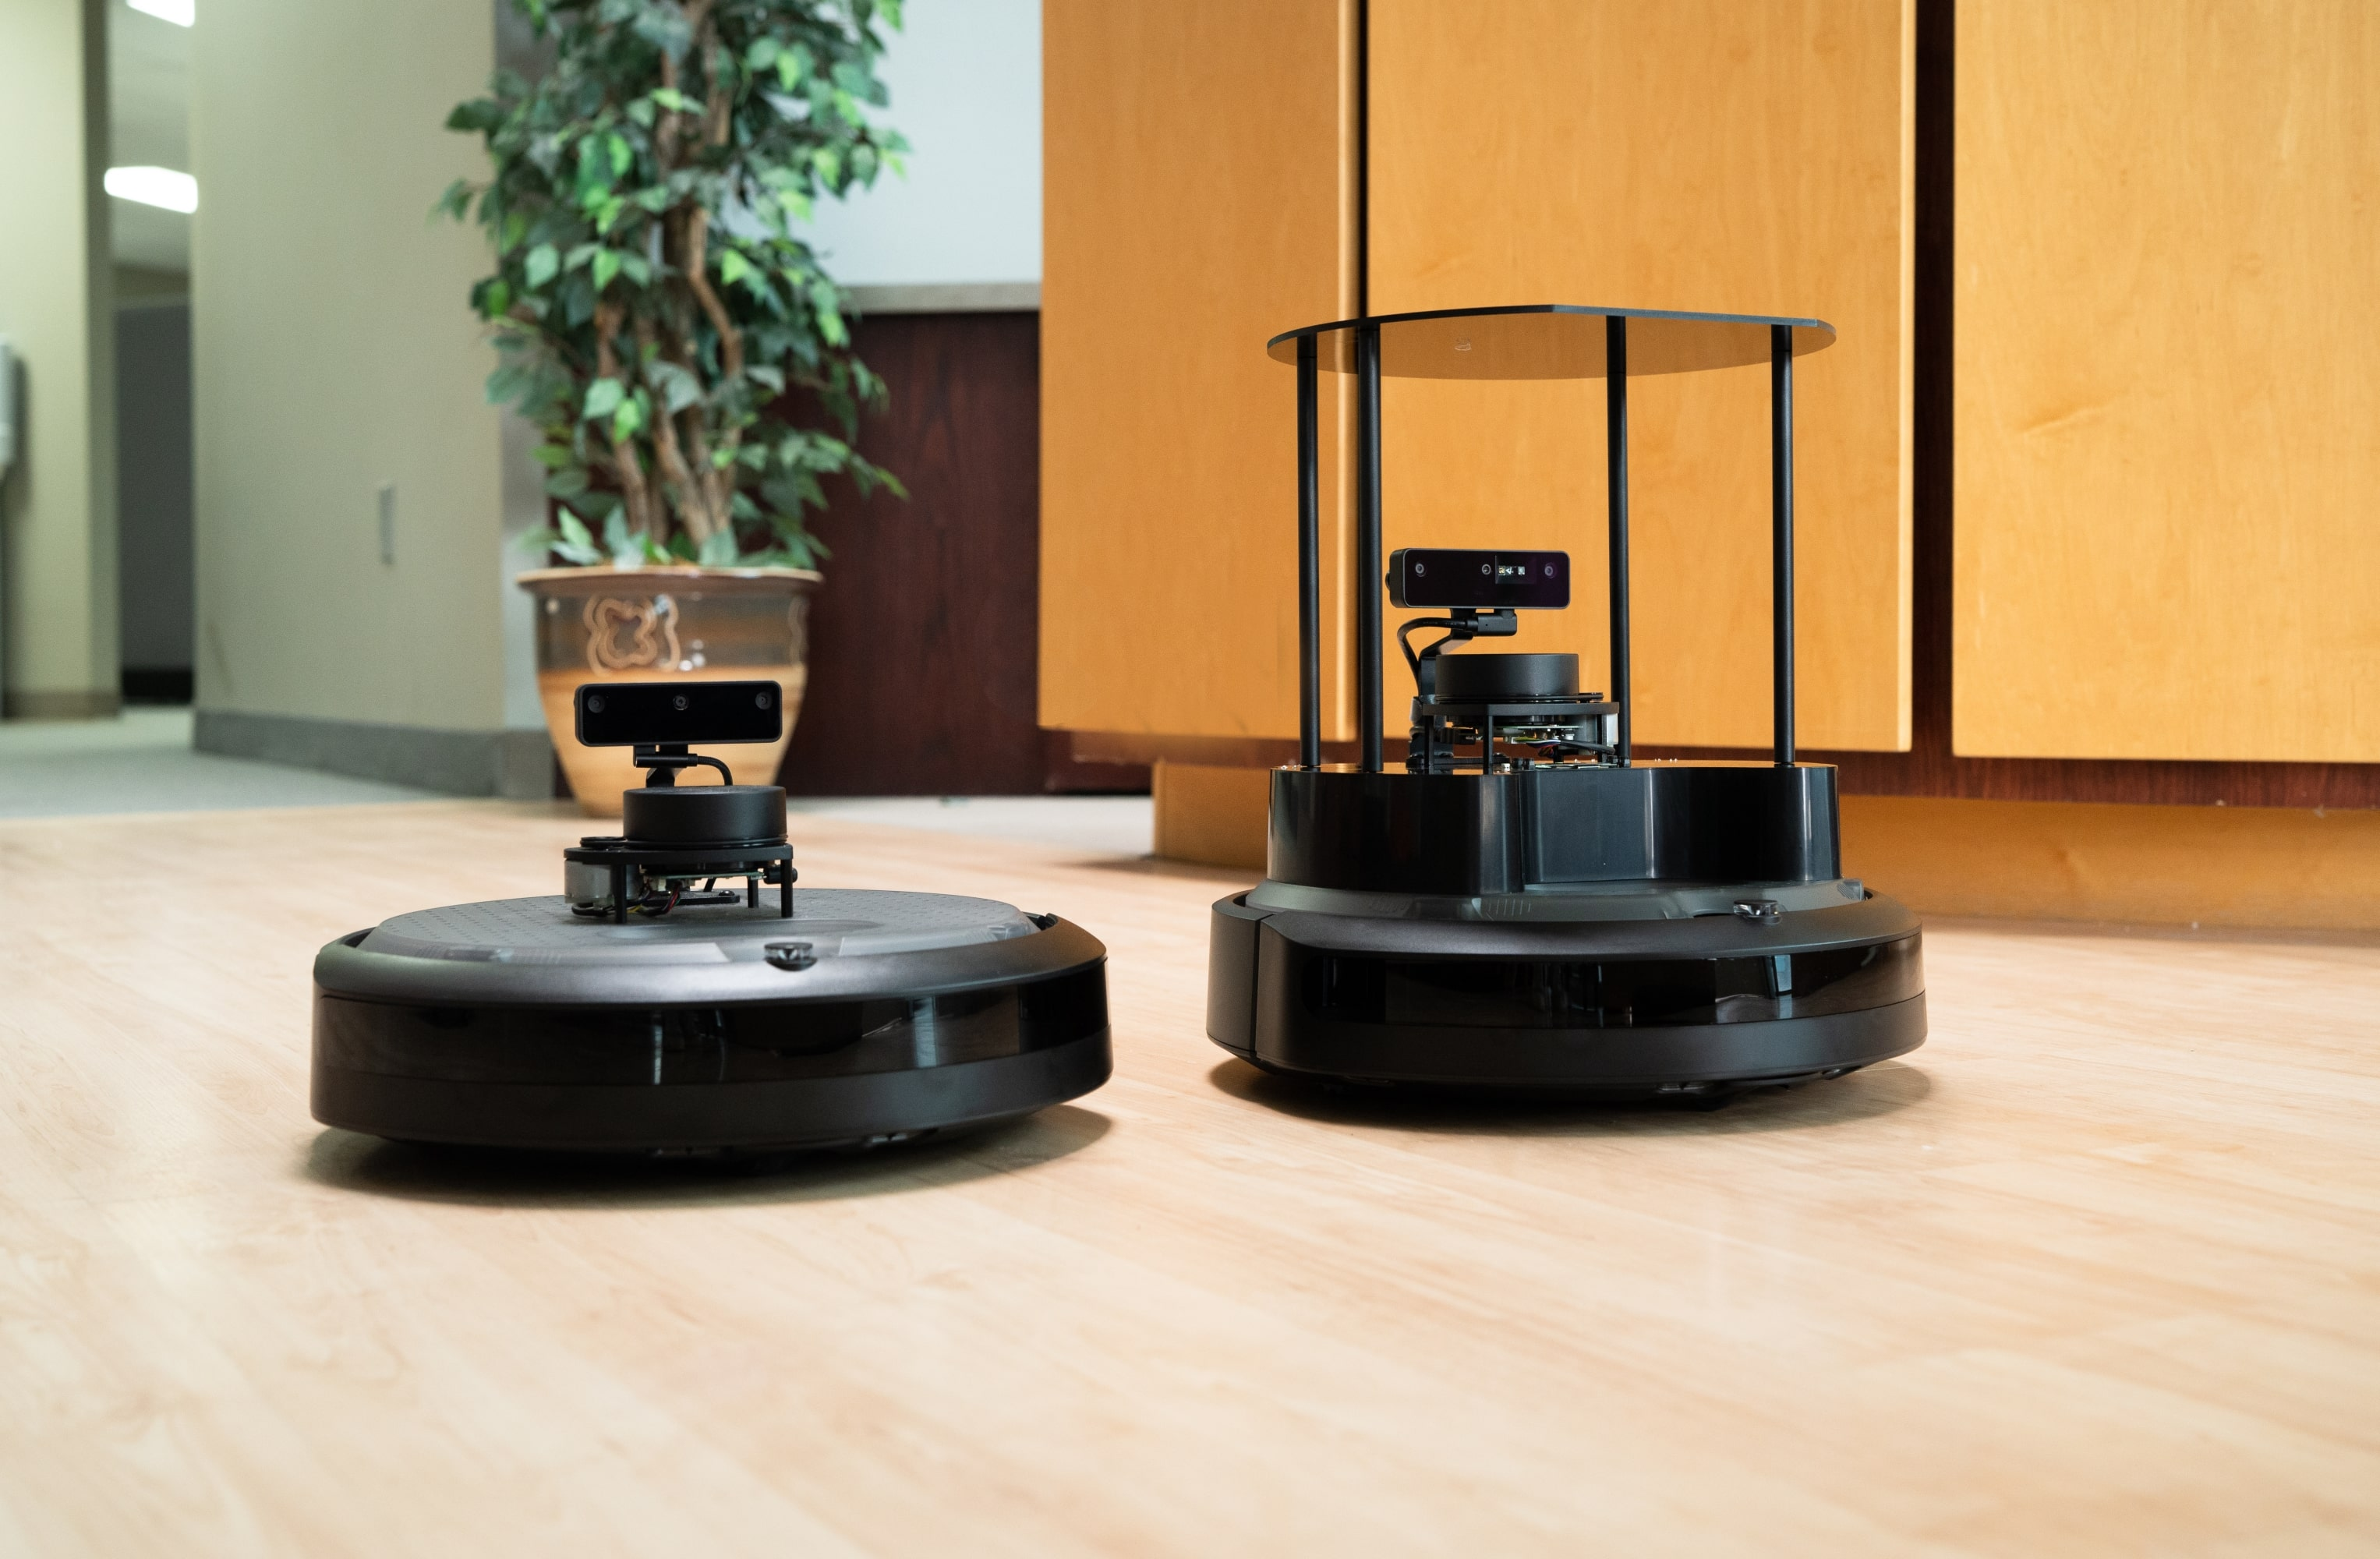
\includegraphics[width=150mm, keepaspectratio]{figures/TurtleBot4.jpg}
    \caption{Turtlebot4 Lite (left) and Turtlebot4 (source:\cite{Turtlebot4Pic})}
    \label{fig:turtlebot4}
\end{figure}

\subsection{Raspberry Pi 4}

Raspberry Pi 4\footnote{\url{https://www.raspberrypi.com/products/raspberry-pi-4-model-b/}} is a mini PC which can be used in various applications:
\begin{itemize}
    \item at home as a desktop PC,
    \item as a NAS (Network-Attached Storage),
    \item as a media server,
    \item in complex embedded systems,
    \item in mobile robots.
\end{itemize}
The device is equipped with a quad core ARM v8 Cortex-A72\footnote{\url{https://www.arm.com/products/silicon-ip-cpu/cortex-a/cortex-a72}} 64-bit SoC, Gigabit ethernet, 2 micro-HDMI ports which support resolution up to 4K, an USB-C power input and 2, 4 or 8 GB of RAM (it can be chosen by our needs or budget). In the Turtlebot4 the Raspberry Pi is used to run ROS2.


\subsection{RPLIDAR-A1}

The Turtlebot4 is equipped with an RPLIDAR-A1\footnote{\url{https://www.slamtec.ai/product/slamtec-rplidar-a1/}} by Slamtech. It is a 2D LIDAR which can scan its surroundings up to 12 meters in 360°. Its maximum resolution is 1° with a maximum sampling frequency of 1 Hz.

The sensor is fully plug-and-play, it has a USB interface, open-source SDK and (thankfully) ROS integration. It goes without saying, but it is worth noting that it meets the Class 1 laser safety standard and is completely safe for human eyes\cite{LaserSafety}.

\subsection{OAK-D Pro}

OAK\footnote{\url{https://shop.luxonis.com/collections/oak-cameras-1}} is a robotic vision camera series made by Luxonis\footnote{\url{https://www.luxonis.com/}}. On the Turtlebot4 sits an OAK-D Pro model and I got an OAK-D model from Nokia to test my implementations at home.

First let's review the specifics of the OAK-D:
\begin{itemize}
    \item it has an IMX378 color camera,
    \item a pair of OV9282 as the stereo cameras (grayscale),
    \item an integrated 9-axis IMU,
    \item a VPU that can run neural network models.
\end{itemize}

Then the OAK-D Pro:
\begin{itemize}
    \item it has an IMX378 Auto-Focus color camera,
    \item a pair of OV9282 as stereo cameras (greyscale),
    \item it supports active stereo,
    \item it has IR illumination for night vision.
\end{itemize}
The active stereo\cite{Stereo} is quite interesting, let's review it in a few words. Passive stereo uses the two cameras to calculate the distances between the camera and the objects thus we can create a 3D map or point cloud of our surroundings with it. This method works optimally in environments with diverse surfaces because it can only calculate the distances if the two cameras can see the exact same points on their images. In case we point the camera to a monotonous surface (for example a clean white wall) it will not be able to calculate the distances due to the miss of matching points. On the contrary, active stereo cameras project a dot matrix so they are able to find matching points even on monotonous surfaces.

\begin{figure}[H]
    \centering
    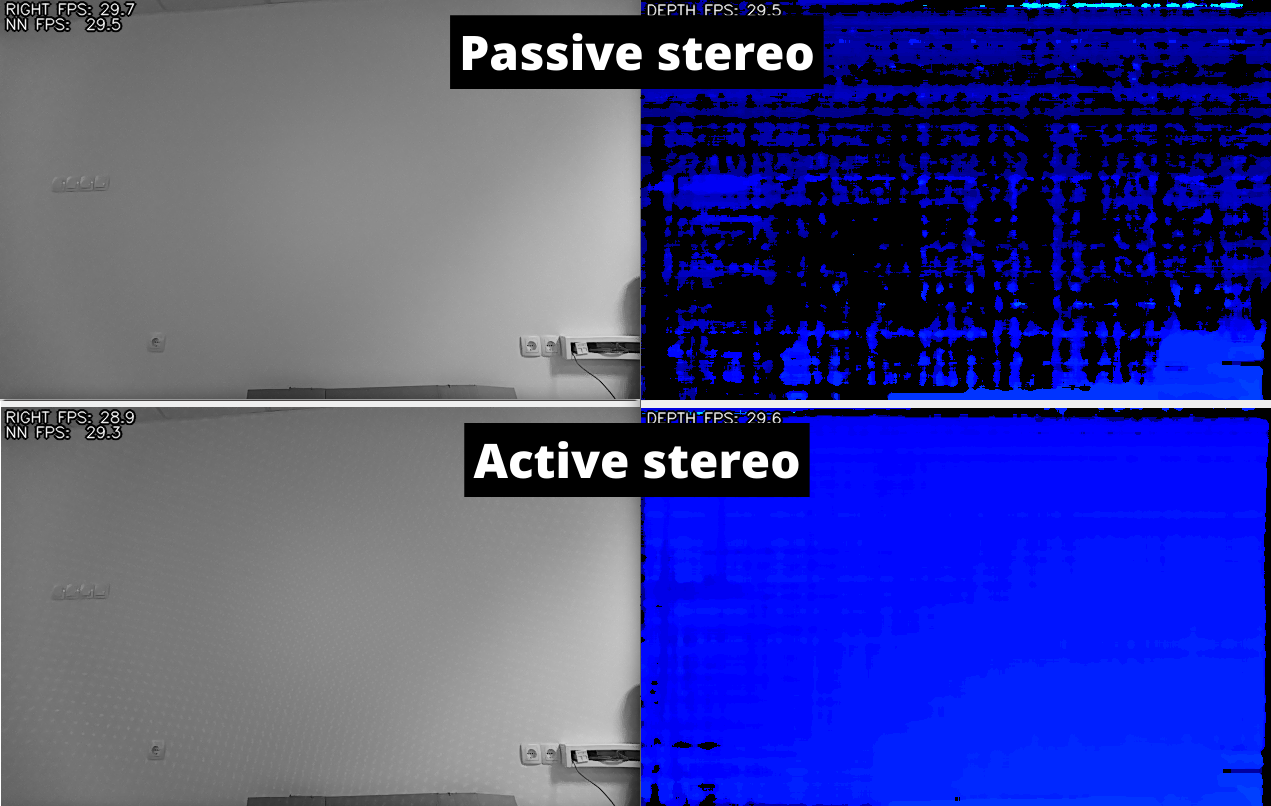
\includegraphics[width=150mm, keepaspectratio]{figures/active-vs-passive-stereo.png}
    \caption{Passive vs active stereo feature matching (source:\cite{ActivePassiveStereo})}
    \label{fig:active-passive-stereo}
\end{figure}

\section{Spectacular AI}

Spectacular AI\footnote{\url{https://www.spectacularai.com/}} provides an SDK\footnote{\url{https://github.com/SpectacularAI/sdk}} for OAK cameras that can be used for various applications:
\begin{itemize}
    \item camera's image visualization,
    \item IMU's localization visualization,
\end{itemize}
The main goal of the SDK is to lend us a hand when we want to do SLAM with an OAK camera. It supports working with ROS through some basic ROS nodes and bridges. The SDK's main strenght is the usage of the IMU and VPU in the OAK camera.

\section{Gaussian Splatting}

